%%
%% Results
%%

\chapter{Results}

This chapter summarizes the four demonstrations held in class on January 24, 2012. The main goal of this
demonstrations was to show data collecting \acp{VV} carried by \acp{RV}, as well as \acp{VV} migrating
among \acp{RV}. All images shown in this chapter were rendered by utilizing Google Maps \cite{GOOGLEMAPS} in a web browser.


\section{Demonstration 1: Data Collection}
In this demonstration one flying \ac{RV} carries one \ac{VV}, which collects data at four locations.
\begin{figure}[h]
	\begin{center}
		\begin{tabular}{cc}
			a)&{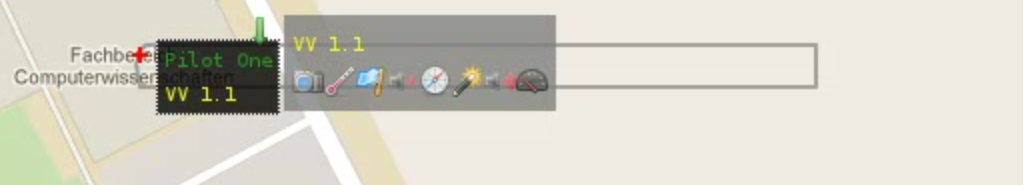
\includegraphics[width=9.4cm]{ese-demo1-1.png}} \\
			b)&{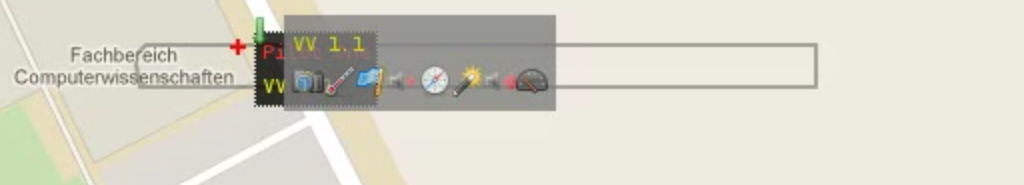
\includegraphics[width=9.4cm]{ese-demo1-2.png}} \\
			
			c)&{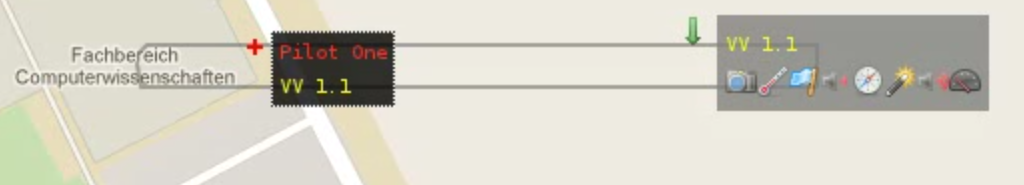
\includegraphics[width=9.4cm]{ese-demo1-3.png}} \\
			d)&{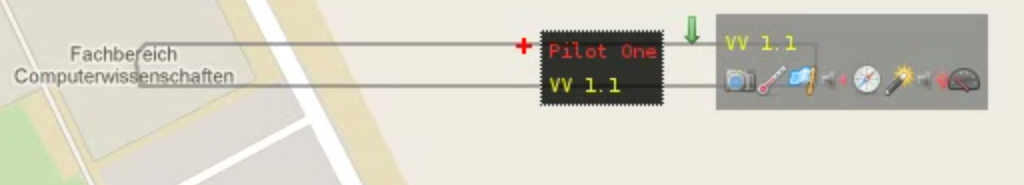
\includegraphics[width=9.4cm]{ese-demo1-4.png}} \\
			
			e)&{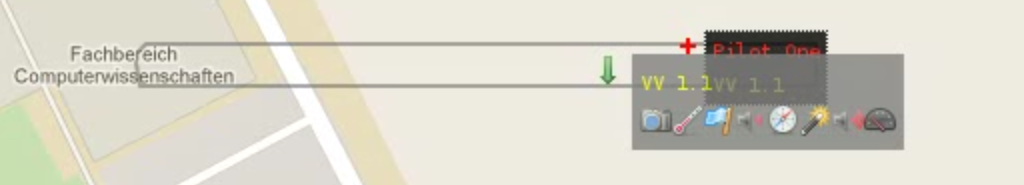
\includegraphics[width=9.4cm]{ese-demo1-5.png}} \\
			f)&{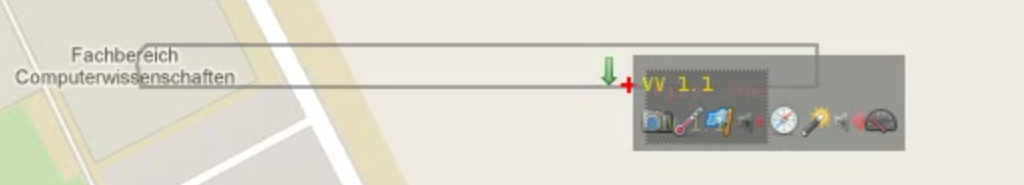
\includegraphics[width=9.4cm]{ese-demo1-6.png}} \\
	
			g)&{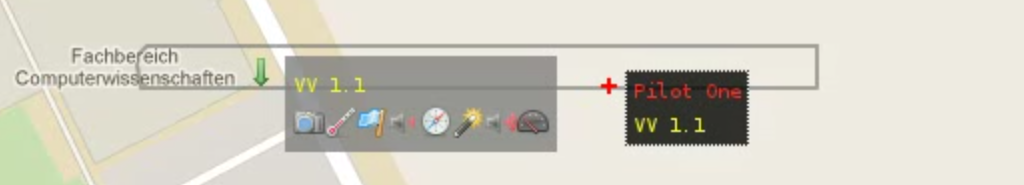
\includegraphics[width=9.4cm]{ese-demo1-7.png}} \\
			h)&{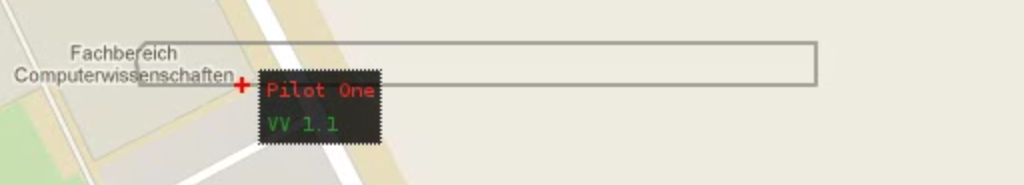
\includegraphics[width=9.4cm]{ese-demo1-8.png}}
		\end{tabular}
	\end{center}
	\caption{Data Collection Demonstration.\label{fig:demo1}}
\end{figure}
Figure~\ref{fig:demo1}~a displays \ac{RV} \textit{Pilot~One} with \ac{VV} \textit{VV~1.1} onboard.
The color green of \textit{Pilot~One} indicates that the \ac{RV} is still on the ground, and the
color yellow of \textit{VV~1.1} shows that the \ac{VV} still has action points to process.
The action points of \textit{VV~1.1} comand accessing the sensors belly mounted photo camera, thermometer,
barometer, sonar, course over ground, random, GPS altitude, and speed over ground. 
In Figure~\ref{fig:demo1}~b \textit{Pilot~One} approaches the first action point. The red label indicates
that the \ac{RV} is flying. After completing the first action point \textit{Pilot~One} approaches the
second action point of \textit{VV~1.1}, as depicted in Figures~\ref{fig:demo1}~c and \ref{fig:demo1}~d.
Figures~\ref{fig:demo1}~e, \ref{fig:demo1}~f, and \ref{fig:demo1}~g visualize \textit{Pilot~One} heading
for the third and fourth action point. After processing the fourth action point, the \ac{VV}'s label
becomes green, which denotes the completion of \textit{VV~1.1}'s mission.

\section{Demonstration 2: Migration}
In this demonstration two \acp{RV} fly along their set courses and one \ac{VV} collects data at five locations.
The blue line in Figure~\ref{fig:demo2vvPath} suggests the virtual path of vehicle \textit{VV~2.1}.
\begin{figure}[h]
	\begin{center}
		{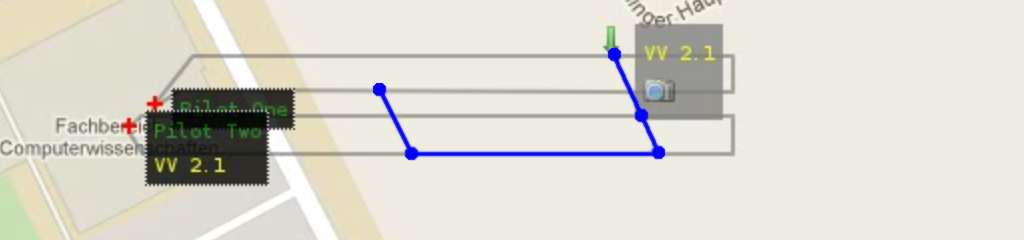
\includegraphics[width=9.4cm]{ese-demo2-1.png}}
	\end{center}
	\caption{Path of Virtual Vehicle \textit{VV~2.1}.\label{fig:demo2vvPath}}
\end{figure}
Initially, \ac{RV} \textit{Pilot~Two} carries \textit{VV~2.1}. After the \acp{RV} take off, a migration
of \textit{VV~2.1} from \textit{Pilot~Two} to \textit{Pilot~One} must take place to allow the \ac{VV} to
reach the first action point. The currently available mapping algorithm considers only the current
set course segment of a \ac{RV} for mapping decisions.
In this demonstration the first action point resides on the second segment of the  set course of
\textit{Pilot~One}. As displayed in Figure~\ref{fig:demo2mig01}, the mapper migrates \textit{VV~2.1} as
soon as \textit{Pilot~One} enters its second set course segment. 
\begin{figure}[h]
	\begin{center}
		{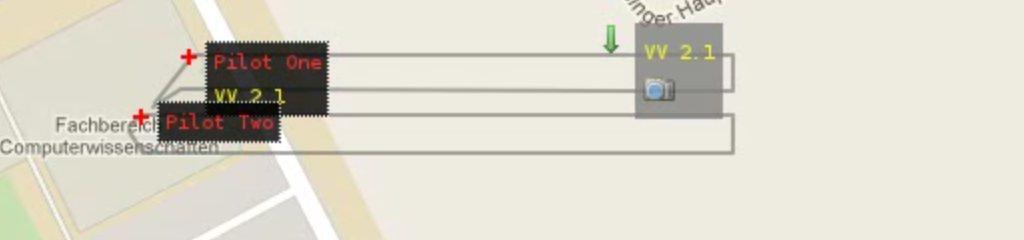
\includegraphics[width=9.4cm]{ese-demo2-2.png}}
	\end{center}
	\caption{First migration of \textit{VV~2.1} from \textit{Pilot~Two} to \textit{Pilot~One}
	initiated by a decision of the mapping algorithm.\label{fig:demo2mig01}}
\end{figure}
\textit{VV~2.1} resides on \textit{Pilot~One} until the \ac{RV} reaches the first action point
(Figure~\ref{fig:demo2mig02}~a). As soon as \textit{VV~2.1} has captured an image via the belly mounted camera,
the mapping algorithm decides to initiate a migration of the \ac{VV} to \textit{Pilot~Two}
(Figure~\ref{fig:demo2mig02}~b). Then, \textit{VV~2.1} takes a picture on the second action point.  
%
Now, there are no action points in the current set course segments of both \acp{RV}. In such a case
the currently implemented mapping algorithm can not decide whether migrating the \ac{VV} would be
benificious or not. So, the \ac{VV} stays on board of \textit{Pilot~Two} until the mapping algorithm
decides otherwise.
%
\begin{figure}[h]
	\begin{center}
		\begin{tabular}{rr}
			a)&{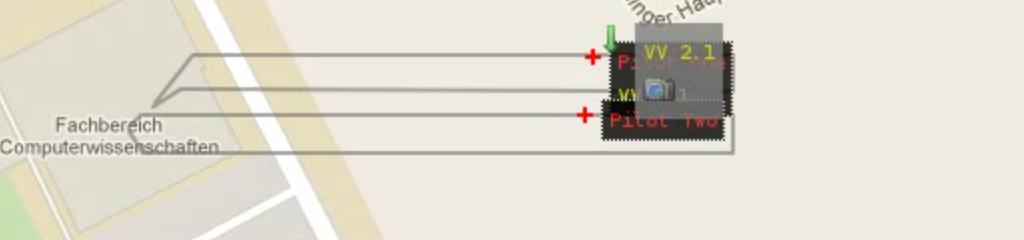
\includegraphics[width=9.4cm]{ese-demo2-3.png}} \\
			b)&{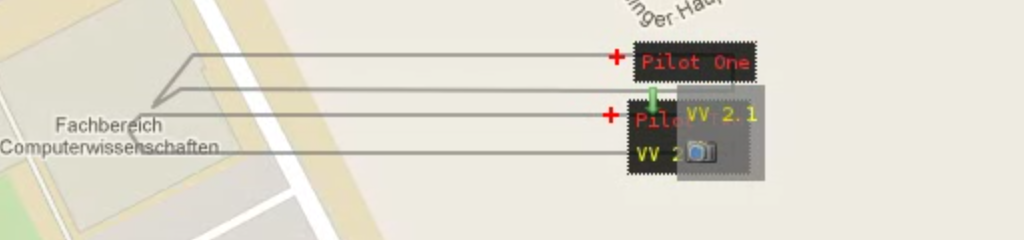
\includegraphics[width=9.4cm]{ese-demo2-4.png}} \\
			c)&{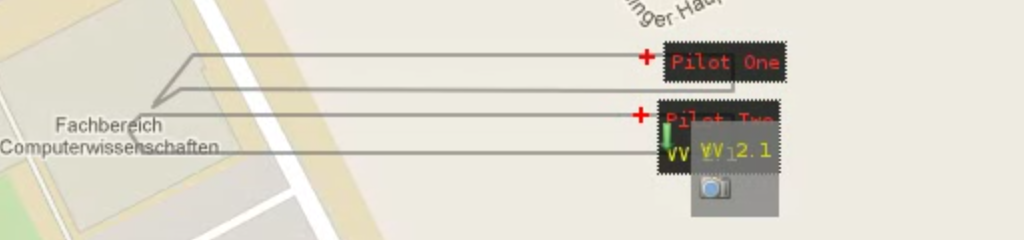
\includegraphics[width=9.4cm]{ese-demo2-5.png}} \\
			d)&{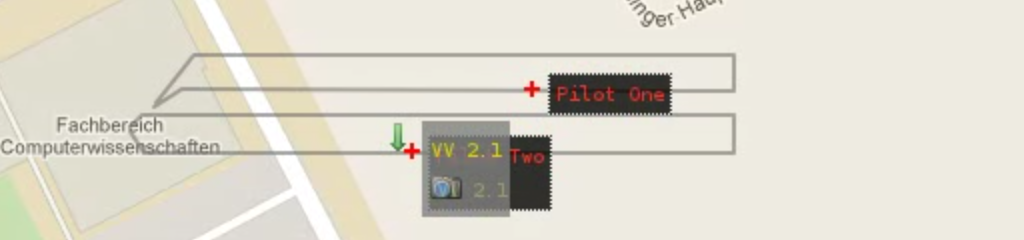
\includegraphics[width=9.4cm]{ese-demo2-6.png}} \\
			e)&{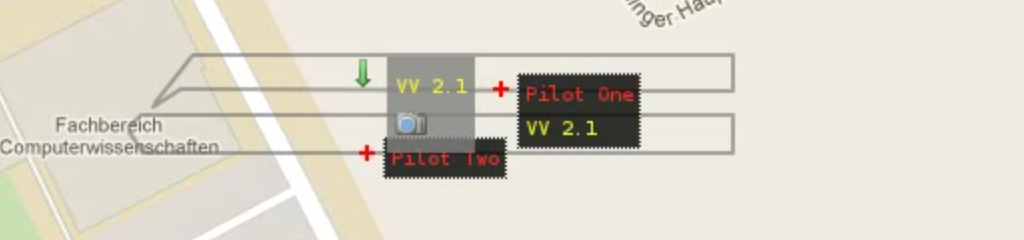
\includegraphics[width=9.4cm]{ese-demo2-7.png}} \\
			f)&{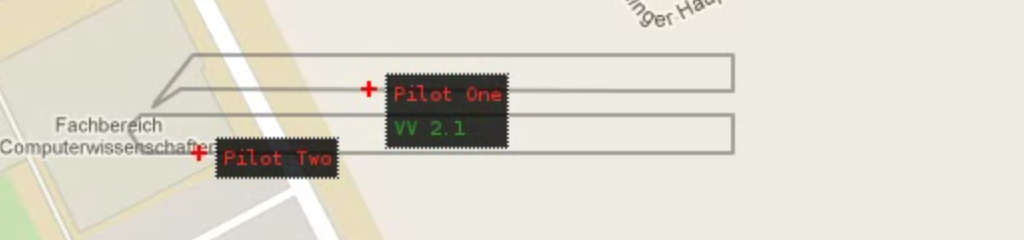
\includegraphics[width=9.4cm]{ese-demo2-8.png}}
		\end{tabular}
	\end{center}
	\caption{\textit{Pilot~One} and \textit{Pilot~Two} mutually carrying \textit{VV~2.1}
		caused by migration decisions of the mapping algorithm.\label{fig:demo2mig02}}
\end{figure}
The \acp{RV} continue to traverse their set courses until \textit{Pilot~Two} enters the fourth segment.
The mapping algorithm detects that \textit{VV~2.1} already is onboard \textit{Pilot~Two} and suppresses
a migration. In Figures~\ref{fig:demo2mig02}~c and \ref{fig:demo2mig02}~d \textit{VV~2.1} captures
photos at the third and at the fourth action point.
%
For the fifth action point, the mapping algorithm decides a migration of \textit{VV~2.1} back to
\textit{Pilot~One}, as visualized in Figure~\ref{fig:demo2mig02}~e. After taking a picture at the last
action point, \textit{VV~2.1} has completed its mission. To indicate this, the label of \textit{VV~2.1}
turns green (Figure~\ref{fig:demo2mig02}~f).
Finally, the mapping algorithm decides a migration back to the central Engine.


\section{Demonstration 3: Different Sensors}
The \acp{RV} in this demonstration do not have the same set of sensors. The first \ac{RV}, \textit{Pilot~One},
carries a thermometer, the second \ac{RV}, \textit{Pilot~Two}, ferries a barometer, and the third \ac{RV},
\textit{Pilot~Three}, transports a belly mounted camera.
All three \acp{RV} follow the same set course in sequence and keep a flying distance of \unit{10}{\second}.
The tasklist of \textit{VV~3.1} consists of two action points, which require capturing photos, temperature
values, and air pressure values.   

Figure~\ref{fig:demo3mig03}~a shows all three \acp{RV} approaching the first action point. Since
\textit{Pilot~One} arrives first and provides a required thermometer sensor, the mapper algorithm already
initiated a migration of \textit{VV~3.1} to \textit{Pilot~One}. 
%
At this point in time, the indicator of the first action point visualizes all three required actions
as incomplete.
%
After \textit{VV~3.1} has completed the temperature measurement, \textit{Pilot~Two} is the next in line
to reach the action point supplying a fitting sensor. Therefore, the mapping algorithm commands a migration 
to \textit{Pilot~Two}.
%
As shown in Figure~\ref{fig:demo3mig03}~b, the action point indicator no more views
the thermometer.
\begin{figure}[h]
	\begin{center}
		\begin{tabular}{rr}
			a)&{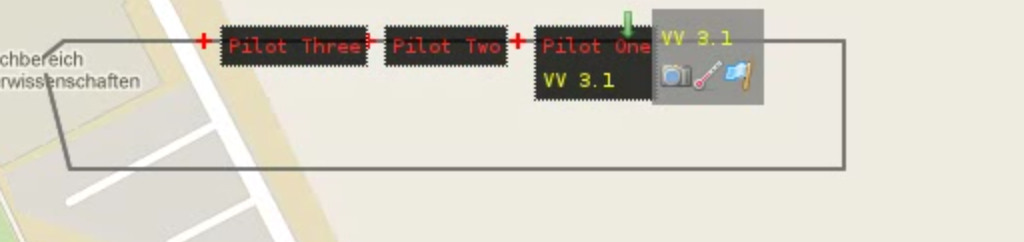
\includegraphics[width=9.4cm]{ese-demo3-1.png}} \\
			b)&{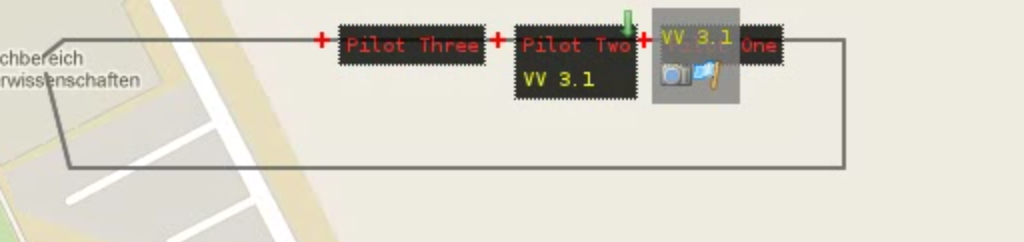
\includegraphics[width=9.4cm]{ese-demo3-2.png}} \\
			c)&{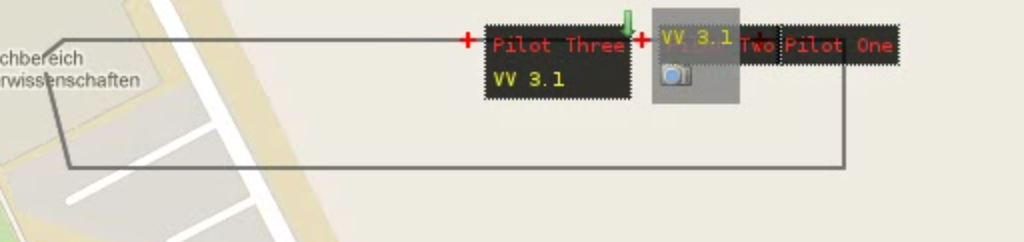
\includegraphics[width=9.4cm]{ese-demo3-3.png}} \\
			d)&{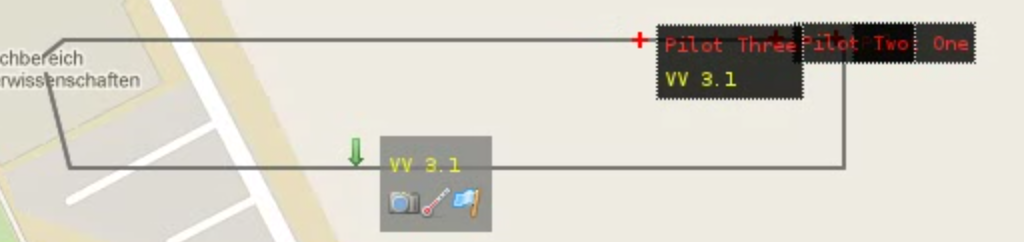
\includegraphics[width=9.4cm]{ese-demo3-4.png}}
		\end{tabular}
	\end{center}
	\caption{\acp{RV} \textit{Pilot~One}, \textit{Pilot~Two}, and \textit{Pilot~Three} mutually carrying
	 	\textit{VV~3.1} repeatedly to the first action point caused by migration decisions of the mapping
	 algorithm.\label{fig:demo3mig03}}
\end{figure}

Figure~\ref{fig:demo3mig03}~c presents the situation after \textit{VV~3.1} has measured the air pressure.
The mapper algorithm already ordered a migration of \textit{VV~3.1} to \textit{Pilot~Three} and
the action point indicator views the remaining action for taking a photo. 
%
Then, \textit{VV~3.1} stays onboard of \textit{Pilot~Three}, because the mapping algorithm can not find
a eligible \ac{RV} for processing the next action point. 

In Figure~\ref{fig:demo3mig04}~a \textit{Pilot~One} enters a set course segment that leads to the next
action point. Since \textit{Pilot~One} faciliates an adequate sensor and is the first to reach the action
point, the mapper algorithm directs a migration of \textit{VV~3.1} to \textit{Pilot~One}.

As \textit{Pilot~One} catches the action point, \textit{VV~3.1} queries the thermometer and the mapper
algorithm orders a migration to \textit{Pilot~Two} (Figure~\ref{fig:demo3mig04}~b).
Again, the action point indicator no more views the thermometer.

\begin{figure}[h]
	\begin{center}
		\begin{tabular}{rr}
			a)&{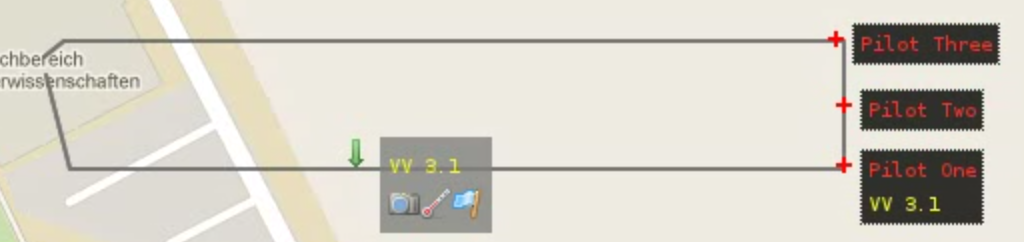
\includegraphics[width=9.4cm]{ese-demo3-5.png}} \\
			b)&{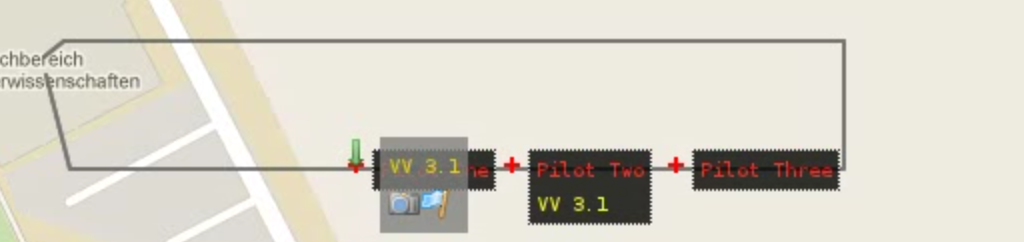
\includegraphics[width=9.4cm]{ese-demo3-6.png}} \\
			c)&{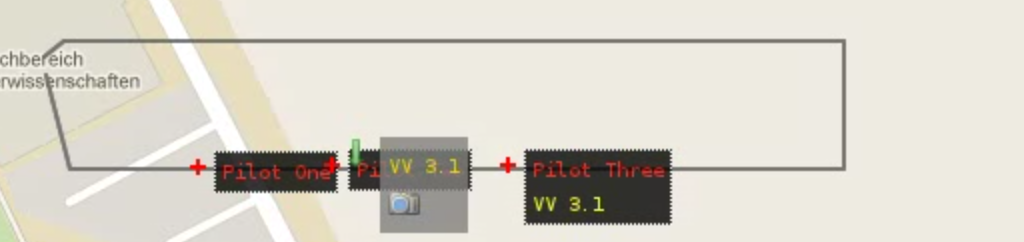
\includegraphics[width=9.4cm]{ese-demo3-7.png}} \\
			d)&{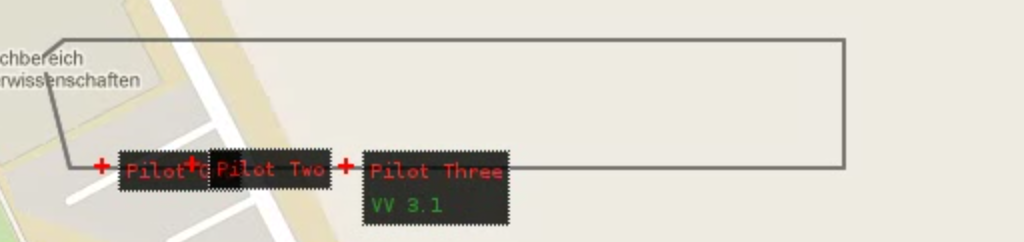
\includegraphics[width=9.4cm]{ese-demo3-8.png}}
		\end{tabular}
	\end{center}
	\caption{\acp{RV} \textit{Pilot~One}, \textit{Pilot~Two}, and \textit{Pilot~Three} mutually carrying
		\textit{VV~3.1} repeatedly to the second action point caused by migration decisions of the mapping
		algorithm.\label{fig:demo3mig04}}
\end{figure}
After that, \textit{Pilot~Two}
arrives at the action point, \textit{VV~3.1} measures the air pressure and the mapper algorithm commands
a migration to \textit{Pilot~Three} (Figure~\ref{fig:demo3mig04}~c).
Consequently, the air pressure symbol vanishes from the action point indicator.
%
Now, \textit{Pilot~Three} gets to the action point and \textit{VV~3.1} completes its mission by 
taking a picture, as shown in Figure~\ref{fig:demo3mig04}~d. The \ac{VV}'s label turns green to show this.

At last, the mapping algorithm initiates a migration back to the central Engine.


\section{Demonstration 4: Multiple Virtual Vehicles}
In this demonstration three \acp{RV} fly along their set courses and four \acp{VV} collect data at several locations.
Each \ac{RV} provides the same set of sensors. Initially, the \acp{VV} idle on the central Engine and wait for
the mapping algorithm to assign an eligible \ac{RV}.  
%
The blue lines in Figure~\ref{fig:demo4img1} display the virtual paths of the \acp{VV}.
All \ac{VV} paths progress top-down, as indicated by black arrows.

Figure~\ref{fig:demo4img1} shows an advanced stage of this demonstration mission displaying all four \acp{VV} in action.
\begin{figure}[h]
	\begin{center}
		{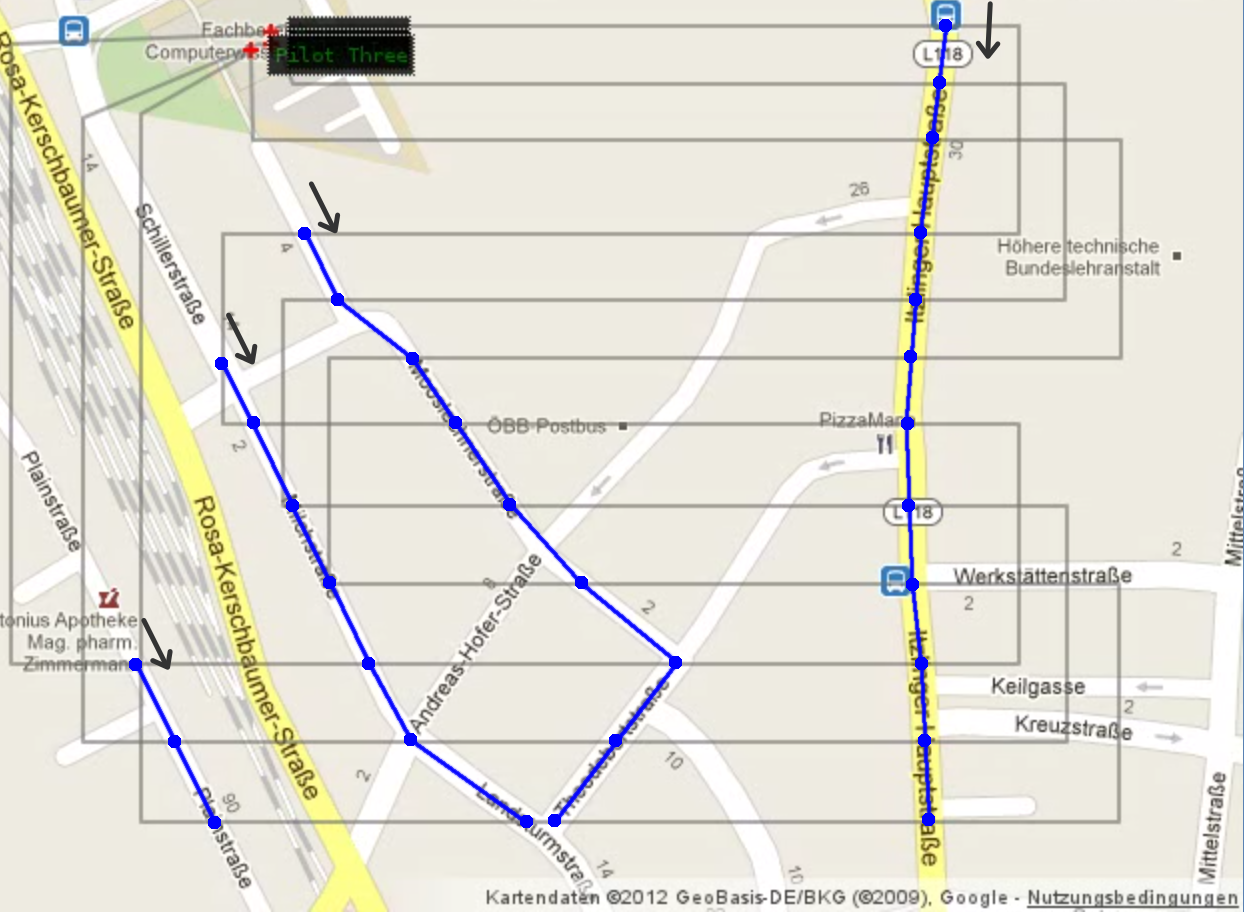
\includegraphics[width=11.42cm]{ese-demo4-1.png}}
	\end{center}
		\caption{Demonstration 4: Virtual Vehicle Paths.\label{fig:demo4img1}}
\end{figure}


\begin{figure}[h]
	\begin{center}
		{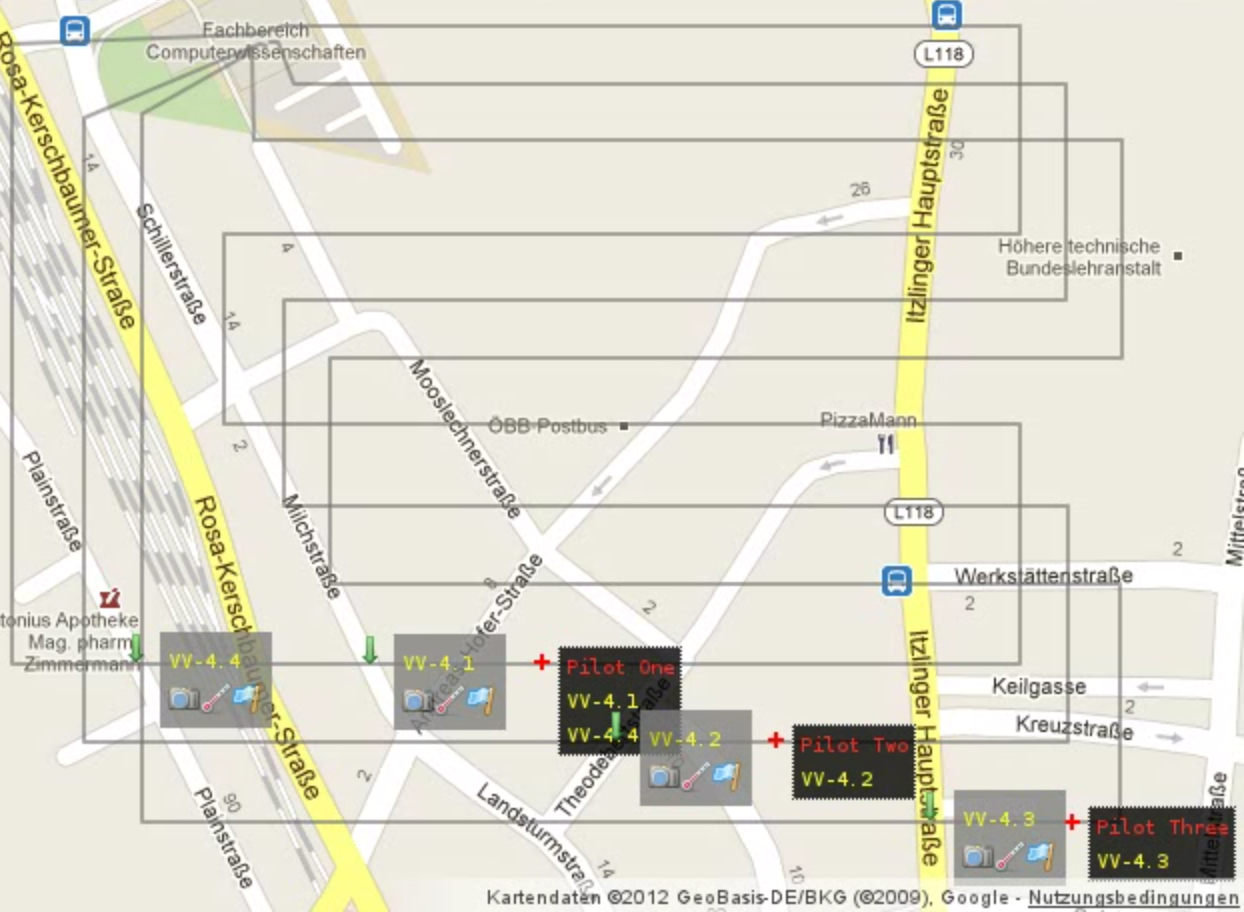
\includegraphics[width=11.42cm]{ese-demo4-2.png}}
	\end{center}
		\caption{Demonstration 4: Multiple \acsp{VV} in action.\label{fig:demo4img2}}
\end{figure}

